\documentclass[spanish]{beamer}
\usepackage[ansinew]{inputenc} % Acepta caracteres en castellano
\usepackage[spanish]{babel}    % silabea palabras castellanas
\usepackage{amsmath}
\usepackage{amsfonts}
\usepackage{amssymb}
\usepackage{dsfont}
\usepackage{graphicx}
\usepackage{geometry}
\usetheme{Madrid}
\usecolortheme{beaver}
\usepackage{textpos}
% Logo  en el comienzo 
\addtobeamertemplate{frametitle}{}{%
\begin{textblock*}{100mm}(.85\textwidth,-1cm)
{\includegraphics[height=0.4in, keepaspectratio=true]{/Users/luisnunez/Dropbox/MisDocumentos/UIS/UISImagenInstitucional/UISLOGO.png}}
\end{textblock*}}

\begin{document}

\title{\textbf{Simetr�as y cantidades conservadas} }
\author[L.A. N��ez]{\textbf{Luis A. N��ez}}  
\institute[UIS]{\textit{Escuela de F�sica, Facultad de Ciencias, } \\
\textit{Universidad Industrial de Santander, Santander, Colombia } \\
{\includegraphics[height=0.4in, keepaspectratio=true]{/Users/luisnunez/Dropbox/MisDocumentos/UIS/UISImagenInstitucional/UISLOGO.png}}
}
\date{\today}
\maketitle


\begin{frame}
\frametitle{Agenda}
  \tableofcontents
\end{frame}


%%%%% Diapo 1
\section{Variables conjugadas y c�clicas}
\frame{
  \frametitle{Variables conjugadas y c�clicas}
   \begin{itemize}  
  	\item<1->  Dado un sistema caracterizado por un Lagrangiano $\mathcal{L}\left(q_j, \dot{q}_j, t\right)$, se define el momento conjugado, $p_j\left(q_j, \dot{q}_j, t\right) \equiv \frac{\partial \mathcal{L}}{\partial \dot{q}_j}$ asociado a la coordenada generalizada $q_j$. Tambi�n llamado momento can�nico.
	\item<2-> El $p_j$ no necesariamente es el momento lineal. Tambi�n puede corresponder al momento angular o a otra cantidad f�sica.
	\item<3-> Si un Lagrangiano $\mathcal{L}$ de un sistema no contiene expl�citamente una coordenada $q_i$ (puede contener $\dot{q}_i$ y $t$ ), se dice que $q_i$ es una coordenada c�clica o ignorable. 
	\item<4-> Entonces,  el momento conjugado $p_i$ asociado a una coordenada c�clica, $q_i$, es constante. Luego, la cantidad $p_i\left(q_j, \dot{q}_j, t\right)$ es una cantidad conservada, i.e. una primera integral del movimiento.
	\item<5-> Si una coordenada $q_i$ es c�clica, entonces $\frac{\partial \mathcal{L}}{\partial q_i}=0$, y la ecuaci�n de Lagrange para esa coordenada c�clica $q_i$ es $\frac{d}{d t}\left(\frac{\partial \mathcal{L}}{\partial \dot{q}_i}\right)  =\frac{d p_i}{d t}=0 
\Rightarrow p_i  =\text { cte. }$
  
    \end{itemize}
}
%
%%%%% Diapo 2
\section{Ejemplo: Part�cula cono invertido}
\frame{
  \frametitle{Part�cula sobre un cono invertido}
   \begin{itemize}  
  	\item<1-> Consideremos una part�cula que se mueve sobre una supreficie c�nica
	\begin{figure}[t]
		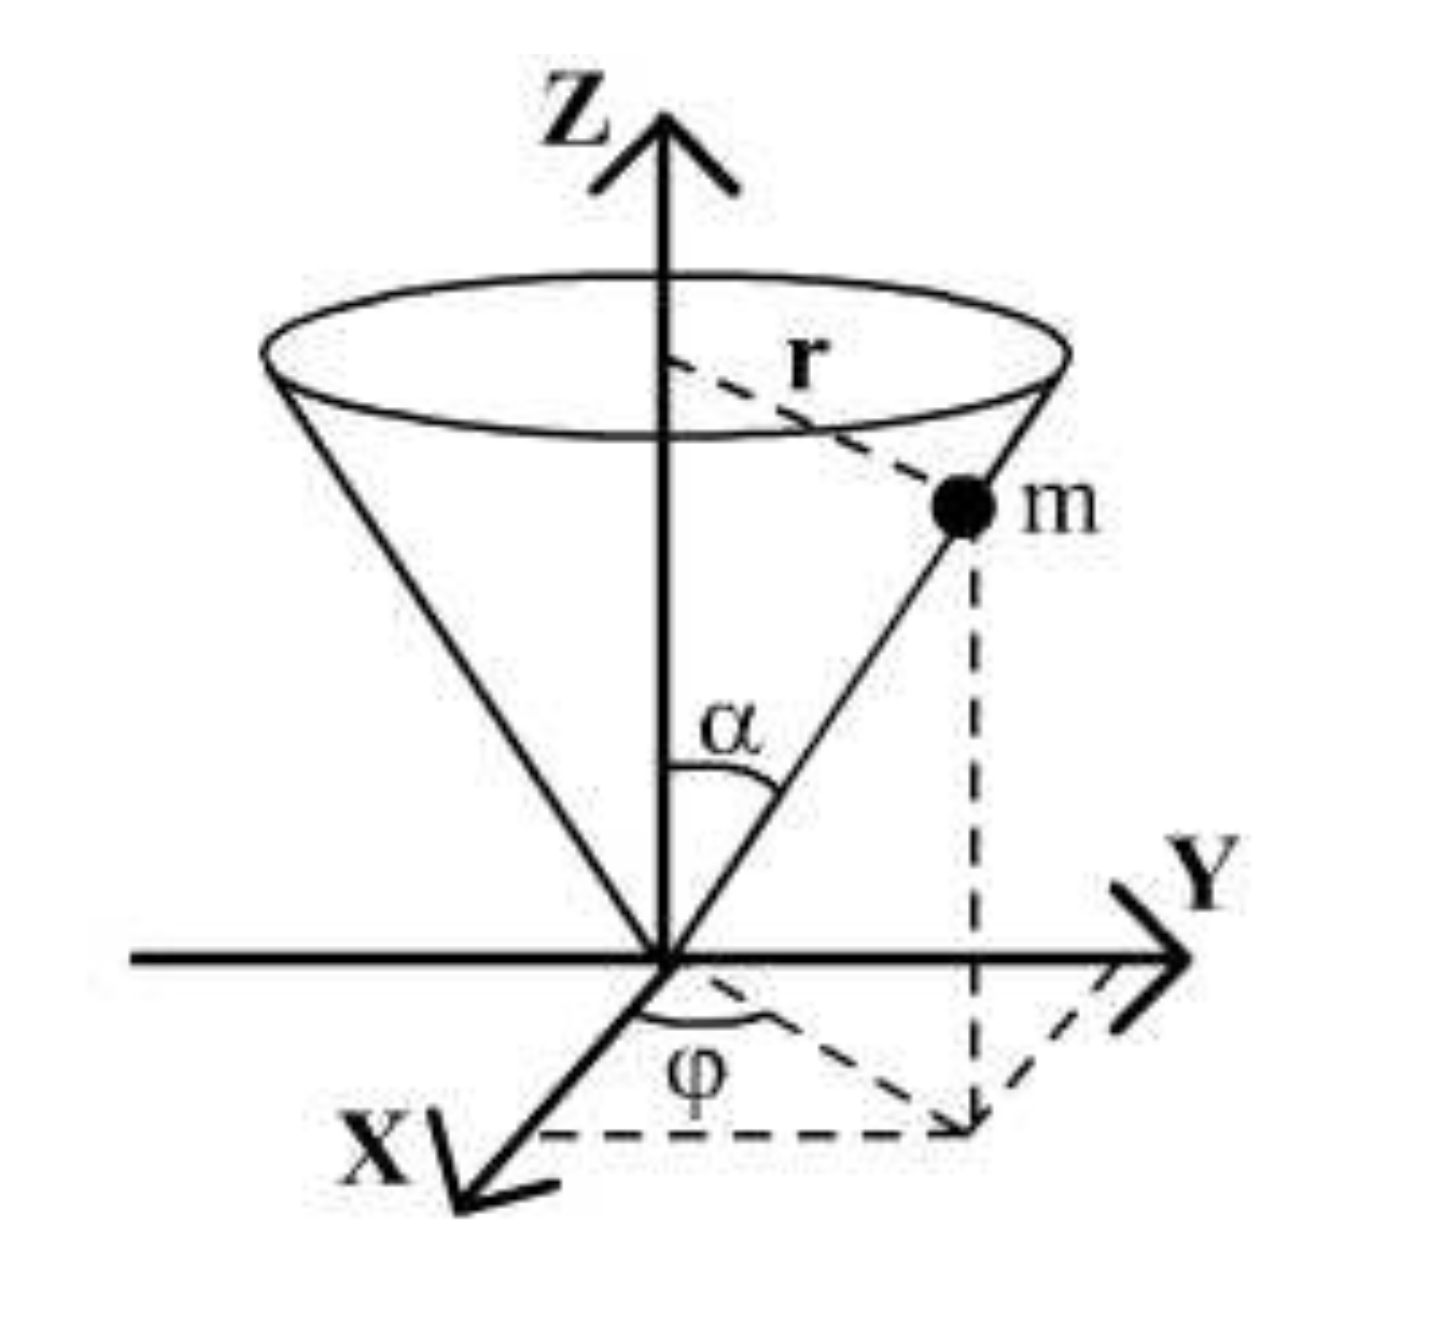
\includegraphics[width=1.0in]{Figuras/Cono.png}
   	\end{figure}
	\item<2-> Su Lagrangeano es  $\mathcal{L}(r, \dot{r}, \dot{\varphi})=\frac{1}{2} m\left(\dot{r}^2 \csc ^2 \alpha+r^2 \dot{\varphi}^2\right)-m g r \cot \alpha$
	\item<3-> La coordenada $\varphi$ es c�clica. El momento conjugado $p_{\varphi}$ asociado con la coordenada angular $\varphi$ es constante, 
	$p_{\varphi}=\frac{ \partial \mathcal{L}}{\partial \dot{\varphi}}=m r^2 \dot{\varphi}=\text { cte }$.
	\item<4-> El momento angular de la part�cula, 
	$\mathbf{L}=\mathbf{r} \times m \mathbf{v} = 
	m\left|\begin{array}{ccc}
		\hat{\mathbf{x}} & \hat{\mathbf{y}} & \hat{\mathbf{z}} \\
		x & y & z \\
		\dot{x} & \dot{y} & \dot{z}
	\end{array}\right| $ 
	\ La componente $z$ es $L_z=m(x \dot{y}-y \dot{x})$

    \end{itemize}
}

%
%%%%% Diapo 2
\section{Secci�n}
\frame{
  \frametitle{T�tulo transparencia}
   \begin{itemize}  
	\item<1-> El momento conjugado $p_r$ asociado a $r$ es $p_r=\frac{ \partial \mathcal{L}}{\partial \dot{r}}=m \dot{r} \csc ^2 \alpha$.
    \end{itemize}
}
%
%%%%% Diapo 2
\section{Secci�n}
\frame{
  \frametitle{T�tulo transparencia}
   \begin{itemize}  
  \item<1-> 
    \end{itemize}
}
%
%%%%% Diapo 2
\section{Secci�n}
\frame{
  \frametitle{T�tulo transparencia}
   \begin{itemize}  
  \item<1-> 
    \end{itemize}
}
%
%%%%% Diapo 2
\section{Secci�n}
\frame{
  \frametitle{T�tulo transparencia}
   \begin{itemize}  
  \item<1-> 
    \end{itemize}
}
%
%%%%% Diapo 2
\section{Secci�n}
\frame{
  \frametitle{T�tulo transparencia}
   \begin{itemize}  
  \item<1-> 
    \end{itemize}
}
%
%%%%% Diapo 2
\section{Secci�n}
\frame{
  \frametitle{T�tulo transparencia}
   \begin{itemize}  
  \item<1-> 
    \end{itemize}
}
%
%%%%% Diapo 2
\section{Secci�n}
\frame{
  \frametitle{T�tulo transparencia}
   \begin{itemize}  
  \item<1-> 
    \end{itemize}
}
  
\end{document}
